% !TEX root = Feuerherdt_Niels_REST_SoSe23.tex
%Einbindung Pakete
\documentclass[11pt,a4paper,oneside]{scrartcl}

%Pakete

%Style
\usepackage[left=2.5cm,right=2.5cm,top=2.0cm,bottom=2.5cm,footskip=1.5cm,head=25pt]{geometry}		
\usepackage{setspace}
\usepackage[bottom,hang]{footmisc}
\usepackage{longtable}

%Sprache
\usepackage[T1]{fontenc}  
\usepackage[utf8]{inputenc}
\usepackage[ngerman]{babel}
\usepackage{eurosym}
\usepackage{lmodern}
\usepackage{blindtext}

%Mathe- Umgebung
\usepackage{amsmath}
\usepackage{amssymb}
\usepackage{amsfonts}

%Grafiken
\usepackage{graphicx}																								
\usepackage{psfrag}
\usepackage{wrapfig}
\usepackage{subfigure}
\usepackage[headsepline,automark]{scrlayer-scrpage}

%Tabellenstil
\usepackage{tabularx}
\usepackage{multirow}
\usepackage{booktabs}
\usepackage{colortbl}
\usepackage[xcdraw]{xcolor}

%Referenzen
\usepackage{url}
\usepackage{hyperref}
\bibliographystyle{unsrt}

%Das hyperref paket führt zu Problemen mit der Internet-Link Darstellung, da bei diesen mit aktivem Paket kein Zeilenumbruch möglich ist ggf. kann hier eine eigene Lösung gefunden werden
%\usepackage[hidelinks]{hyperref}

%Grafikpafad
\graphicspath{{./Abbildungen/}}

%Zusätzliche Pakete
\usepackage{caption}
\usepackage{units}
\usepackage{float}
\usepackage[]{xcolor}
\usepackage{colortbl}
\usepackage{hhline}

%Nachträglich hinzugefügte Pakete
%\usepackage{auto-pst-pdf}


%Initialisierung des Dokuments
\begin{document}

%Einbindung unterschiedlicher Befehlsänderungen
%  Referenzen Befehle
\newcommand{\fref}[1]{Abb. \ref{fig:#1}}
\newcommand{\tref}[1]{Tab. \ref{tab:#1}}
\newcommand{\mref}[1]{(\ref{eq:#1})}
\newcommand{\sref}[1]{Abschnitt \ref{section:#1}}

%Kopfzeile
\ohead[{
\includegraphics[height=20pt]{HTWLogo}}]{
\includegraphics[height=20pt]{HTWLogo}}
\renewcommand*\sectionmarkformat{}

%Farbe
\definecolor{HTWGreen}{cmyk}{0.55, 0.00, 1.00, 0.00}

%Nachträglich hinzugefügte Style Änderungen und Befehlsänderungen



\parindent 0cm

%Zeilenabstand	
\onehalfspacing			 									
\addtolength{\footskip}{-8mm}

%Titelseite
\begin{titlepage}

    \begin{figure}[h] 
            \begin{flushright}
        
\includegraphics[width=0.3\textwidth]{Abbildungen/HTWLogo.eps}\\
            \end{flushright}
    \end{figure}
%    \begin{figure}[h]
%        \centering
%        \includegraphics[width=0.7\textwidth]{Wärmepumpe.png}\\
%    \end{figure}
%Hochschulspezifische Informationen, Hochschule, Fachbereich, Adresse, etc.
\begin{center}
    \vspace*{\fill}
    {\Large Hochschule f{\"u}r Technik und Wirtschaft Berlin}\\
        \bigskip
        Wilhelminenhofstra"se 75A, 12459 Berlin\\
        \bigskip
    Fachbereich 1 \\Ingenieurwissenschaften - Energie und Information\\Regenerative Energien (B)\\
    \vfill
%Versuchspezifische Angaben
     \textcolor{HTWGreen}{\textbf{\Large{Projekt: Planung einer solarthermischen Anlage}}}\\
    \textit{Betreuer: Prof. Dr.-Ing. Friedrich Sick}\\
\vfill
\end{center}
\vfill
%Gruppenmitglieder Liste
\begin{table}[H]
        \centering
        \begin{tabular}{|l|c|}
        \hline
        \rowcolor[cmyk]{0.55, 0.00, 1.00, 0.00} \textbf{Name} & \textbf{Matrikelnummer}  \\
        \hline
        Niels Feuerherdt      & 577669\\
        \hline
        \end{tabular}
        \end{table}
\end{titlepage}

\newpage

%Abstract (dieser ist für Laborprotokolle in der Regel nicht notwendig)
%\input{abstract}
% \newpage

\pagenumbering{roman}

%Inhaltsverzeichnis
\setcounter{tocdepth}{3}
\tableofcontents
\newpage

%Abbildungsverzeichnis, Tabellenverzeichnis und Abkürzungsverzeichnis
\listoffigures
\listoftables
\addtocounter{table}{-1} 
\bigskip
\Large \textsf{\textbf{Abk"urzungsverzeichnis}}
\begin{longtable}{p{2 cm}p{8 cm}} 
\end{longtable}
\newpage
% Please add the following required packages to your document preamble:
% \usepackage{graphicx}
% \usepackage[table,xcdraw]{xcolor}
% If you use beamer only pass "xcolor=table" option, i.e. \documentclass[xcolor=table]{beamer}
\begin{table}[]
    \centering
    \resizebox{1.1\textwidth}{!}{%
    \begin{tabular}{lclcc}
    \cline{1-3}
    \multicolumn{3}{|l|}{\textbf{Projekt REST-Solarthermie, Zusammenfassung}}                                                                                                                                         &                                               &                                               \\ \cline{1-3}
    \multicolumn{3}{|l|}{\textbf{Feuerherdt, Niels}}                                                                                                                                                                  &                                               &                                               \\ \cline{1-3}
                                                                                         &                                                            &                                                               &                                               &                                               \\ \cline{1-3}
    \multicolumn{1}{|l|}{\textbf{Angebot}}                                               & \multicolumn{1}{c|}{\textbf{Wert}}                         & \multicolumn{1}{l|}{\textbf{Einheit}}                         &                                               &                                               \\ \cline{1-3}
    \multicolumn{1}{|l|}{Globalstrahlung horizontal Berlin Mittel}                       & \multicolumn{1}{c|}{1132,47}                               & \multicolumn{1}{l|}{kWh/m²a}                                  &                                               &                                               \\ \cline{1-3}
    \multicolumn{1}{|l|}{Ausrichtungsfaktor}                                             & \multicolumn{1}{c|}{1,05}                                  & \multicolumn{1}{l|}{-}                                        &                                               &                                               \\ \cline{1-3}
    \multicolumn{1}{|l|}{Strahlung in Kollektorebene Mittel}                             & \multicolumn{1}{c|}{1189,09}                               & \multicolumn{1}{l|}{kWh/m²a}                                  &                                               &                                               \\ \cline{1-3}
    \multicolumn{1}{|l|}{Strahlung in Kollektorebene Min.}                               & \multicolumn{1}{c|}{1103,24}                               & \multicolumn{1}{l|}{kWh/m²a}                                  &                                               &                                               \\ \cline{1-3}
    \multicolumn{1}{|l|}{Strahlung in Kollektorebene Max.}                               & \multicolumn{1}{c|}{1305,70}                               & \multicolumn{1}{l|}{kWh/m²a}                                  &                                               &                                               \\ \cline{1-3}
                                                                                         &                                                            &                                                               &                                               &                                               \\ \cline{1-3}
    \multicolumn{1}{|l|}{\textbf{Bedarf}}                                                & \multicolumn{1}{c|}{\textbf{Wert}}                         & \multicolumn{1}{l|}{\textbf{Einheit}}                         &                                               &                                               \\ \cline{1-3}
    \multicolumn{1}{|l|}{Heizwärmebedarf Mittel}                                         & \multicolumn{1}{c|}{8000}                                  & \multicolumn{1}{l|}{kWh/a}                                    &                                               &                                               \\ \cline{1-3}
    \multicolumn{1}{|l|}{Heizwärmebedarf Min.}                                           & \multicolumn{1}{c|}{7712,220}                              & \multicolumn{1}{l|}{kWh/a}                                    &                                               &                                               \\ \cline{1-3}
    \multicolumn{1}{|l|}{Heizwärmebedarf Max.}                                           & \multicolumn{1}{c|}{8287,780}                              & \multicolumn{1}{l|}{kWh/a}                                    &                                               &                                               \\ \cline{1-3}
    \multicolumn{1}{|l|}{WW-Wärmebedarf Mittel}                                          & \multicolumn{1}{c|}{2711,025}                              & \multicolumn{1}{l|}{kWh/a}                                    &                                               &                                               \\ \cline{1-3}
    \multicolumn{1}{|l|}{WW-Wärmebedarf Min.}                                            & \multicolumn{1}{c|}{1355,513}                              & \multicolumn{1}{l|}{kWh/a}                                    &                                               &                                               \\ \cline{1-3}
    \multicolumn{1}{|l|}{WW-Wärmebedarf Max.}                                            & \multicolumn{1}{c|}{4066,538}                              & \multicolumn{1}{l|}{kWh/a}                                    &                                               &                                               \\ \cline{1-3}
    \multicolumn{1}{|l|}{Zirkulationsverluste}                                           & \multicolumn{1}{c|}{8}                                     & \multicolumn{1}{l|}{kWh/a}                                    &                                               &                                               \\ \cline{1-3}
    \multicolumn{1}{|l|}{Gesamtwärmebedarf Mittel}                                       & \multicolumn{1}{c|}{10719,025}                             & \multicolumn{1}{l|}{kWh/a}                                    &                                               &                                               \\ \cline{1-3}
    \multicolumn{1}{|l|}{Gesamtwärmebedarf Min.}                                         & \multicolumn{1}{c|}{9075,733}                              & \multicolumn{1}{l|}{kWh/a}                                    &                                               &                                               \\ \cline{1-3}
    \multicolumn{1}{|l|}{Gesamtwärmebedarf Max.}                                         & \multicolumn{1}{c|}{12362,318}                             & \multicolumn{1}{l|}{kWh/a}                                    &                                               &                                               \\ \cline{1-3}
                                                                                         &                                                            &                                                               &                                               &                                               \\ \hline
    \multicolumn{1}{|l|}{}                                                               & \multicolumn{2}{c|}{\cellcolor[HTML]{9AFF99}\textbf{Mittel}}                                                               & \multicolumn{1}{c|}{\textbf{Extrema A}}       & \multicolumn{1}{c|}{\textbf{Extrema B}}       \\ \hline
    \multicolumn{1}{|l|}{\textbf{Kollektor, Speicher}}                                   & \multicolumn{2}{c|}{\cellcolor[HTML]{9AFF99}Bezeichnung, Anz., Fläche, Volumen}                                            & \multicolumn{1}{c|}{}                         & \multicolumn{1}{c|}{}                         \\ \hline
    \multicolumn{1}{|l|}{gewählter Kollektortyp}                                         & \multicolumn{2}{c|}{\cellcolor[HTML]{9AFF99}Viessmann Vitosol 200-FM}                                                      & \multicolumn{1}{c|}{Viessmann Vitosol 200-FM} & \multicolumn{1}{c|}{}                         \\ \hline
    \multicolumn{1}{|l|}{Anzahl Kollektoren}                                             & \multicolumn{2}{c|}{\cellcolor[HTML]{9AFF99}6}                                                                             & \multicolumn{1}{c|}{5}                        & \multicolumn{1}{c|}{8}                        \\ \hline
    \multicolumn{1}{|l|}{Kollektorfläche}                                                & \multicolumn{2}{c|}{\cellcolor[HTML]{9AFF99}13,86}                                                                         & \multicolumn{1}{c|}{11,55}                    & \multicolumn{1}{c|}{18,48}                    \\ \hline
    \multicolumn{1}{|l|}{gewählter Speichertyp}                                          & \multicolumn{2}{c|}{\cellcolor[HTML]{9AFF99}Viessmann Vitocell 340-M}                                                      & \multicolumn{1}{c|}{Viessmann Vitocell 340-M} & \multicolumn{1}{c|}{Viessmann Vitocell 360-M} \\ \hline
    \multicolumn{1}{|l|}{Speichervolumen}                                                & \multicolumn{2}{c|}{\cellcolor[HTML]{9AFF99}750}                                                                           & \multicolumn{1}{c|}{750}                      & \multicolumn{1}{c|}{950}                      \\ \hline
                                                                                         & \cellcolor[HTML]{9AFF99}                                   & \cellcolor[HTML]{9AFF99}                                      &                                               &                                               \\ \hline
    \multicolumn{1}{|l|}{\textbf{Verrohrung}}                                            & \multicolumn{1}{c|}{\cellcolor[HTML]{9AFF99}\textbf{Wert}} & \multicolumn{1}{l|}{\cellcolor[HTML]{9AFF99}\textbf{Einheit}} & \multicolumn{1}{c|}{\textbf{Wert}}            & \multicolumn{1}{c|}{\textbf{Wert}}            \\ \hline
    \multicolumn{1}{|l|}{Durchmesser DNxx}                                               & \multicolumn{1}{c|}{\cellcolor[HTML]{9AFF99}DIN20}         & \multicolumn{1}{l|}{\cellcolor[HTML]{9AFF99}-}                & \multicolumn{1}{c|}{DIN15}                    & \multicolumn{1}{c|}{DIN20}                    \\ \hline
    \multicolumn{1}{|l|}{Strömungsgeschwindigkeit}                                       & \multicolumn{1}{c|}{\cellcolor[HTML]{9AFF99}0,49}          & \multicolumn{1}{l|}{\cellcolor[HTML]{9AFF99}m/s}              & \multicolumn{1}{c|}{0,64}                     & \multicolumn{1}{c|}{0,65}                     \\ \hline
                                                                                         & \cellcolor[HTML]{9AFF99}                                   & \cellcolor[HTML]{9AFF99}                                      &                                               &                                               \\ \hline
    \multicolumn{1}{|l|}{\textbf{Druckverlust Kollektorfeld, Rohrleitung und Einbauten}} & \multicolumn{1}{c|}{\cellcolor[HTML]{9AFF99}\textbf{Wert}} & \multicolumn{1}{l|}{\cellcolor[HTML]{9AFF99}\textbf{Einheit}} & \multicolumn{1}{c|}{\textbf{Wert}}            & \multicolumn{1}{c|}{\textbf{Wert}}            \\ \hline
    \multicolumn{1}{|l|}{Druckverlust Kollektorfeld Parallelverschaltung}                & \multicolumn{1}{c|}{\cellcolor[HTML]{9AFF99}14500}         & \multicolumn{1}{l|}{\cellcolor[HTML]{9AFF99}Pa}               & \multicolumn{1}{c|}{8000}                     & \multicolumn{1}{c|}{17500}                    \\ \hline
    \multicolumn{1}{|l|}{Druckverlust Rohrleitung}                                       & \multicolumn{1}{c|}{\cellcolor[HTML]{9AFF99}4884,72}       & \multicolumn{1}{l|}{\cellcolor[HTML]{9AFF99}Pa}               & \multicolumn{1}{c|}{9937,98}                  & \multicolumn{1}{c|}{11757,43}                 \\ \hline
    \multicolumn{1}{|l|}{Druckverlust sonstiger Einbauten}                               & \multicolumn{1}{c|}{\cellcolor[HTML]{9AFF99}2198,12}       & \multicolumn{1}{l|}{\cellcolor[HTML]{9AFF99}Pa}               & \multicolumn{1}{c|}{4472,09}                  & \multicolumn{1}{c|}{5290,84}                  \\ \hline
    \multicolumn{1}{|l|}{Gesamtdruckverlust des Kollektorkreises}                        & \multicolumn{1}{c|}{\cellcolor[HTML]{9AFF99}21582,84}      & \multicolumn{1}{l|}{\cellcolor[HTML]{9AFF99}Pa}               & \multicolumn{1}{c|}{22410,08}                 & \multicolumn{1}{c|}{34548,28}                 \\ \hline
    \end{tabular}%
    }
    \caption{Zusammenfassung aller Ergebnisse}
    \label{tab: Summary}
    \end{table}
    \newpage
\clearpage
\pagenumbering{arabic}

%Inhaltlicher Teil
\section{Einleitung}
\label{sec:Einleitung}
Die Auslegung einer Solarthermieanlage bedarf einiger Vertiefungen und Berechnungen.\\
Ziel dieser Betrachtungen ist es, alle Komponenten korrekt zu dimensionieren.
Hierbei werden von Strahlungsbedingungen bis Anlageneingenschaften viele Faktoren mit eingebunden.
Wie eine solche Auslegung annähernd funktionieren kann, zeigt diese Ausarbeitung.


\section{Angebot und Bedarf}
\label{sec:Angebot und Bedarf}
\subsection{a}
Der hinreichend große Anteil des Dachs, der die Kollektoren aufnehmen soll, ist 40° zur Horizontalen
geneigt und nach Süd-Ost orientiert. Bestimmen Sie für den Standort Berlin die jährliche Einstrahlungs-
summe E in kWh/m² in der Kollektorebene aus dokumentierten Daten (DWD, HTW Berlin, einschlägige
Software). Bemühen Sie sich dabei einen langjährigen Mittelwert zu finden und geben Sie eine begrün-
dete Aussage zur Schwankungsbreite um dieses langjährige Mittel
% 𝐸 ± ∆𝐸.
  Erläutern Sie Ihre Vorge-
hensweise.
\subsection{b}
Zur korrekten Dimensionierung der Anlage ist die Betrachtung des Gesamtwärmebedarfs von zentraler Rolle.
Auf den Gesamtwärmebedarf haben vor allem die Dämm- und Speichereigenschaften des Gebäudes, sowie das Nutzungsprofil der Bewohner Einfluss.\\
Für das betrachtete Gebäude werden $160 m^2$ Wohnfläche bei einem spezifischen jährlichen Heizwärmebedarf von $50 \frac{kWh}{m^2 \cdot a}$ angegeben.
Die Multiplikation dieser beiden Werte ergibt für den mittleren Heizwärmebedarf $Q_H = 8000 \frac{kWh}{a}$.\\
Um eine begründete Abschätzung der Schwankungsbreite für diesen Wert zu erhalten, wurden Daten über den Gesamtverbrauch im Bereich "'Space Heating"' in Deutschland von 2012 bis 2021 verwendet.\cite{EuroStat}\\
Mit Hilfe der Berechnung der relativen mittleren Abweichung der Werte konnte eine Toleranzgrenze von $\Delta Q_H = \pm 287,78 \frac{kWh}{a}$ ermittelt werden.\\
\newpage
Anschließend wurde der Warmwasserwärmebedarf $Q_{WW}$ für mittleren, niedrigen und hohen Verbrauch \cite[S.119]{Sick22} berechnet.
Mittels \autoref{eq:Warmwasser} ergab sich für den betrachteten 4-Personen-Haushalt ein mittlerer Warmwasserwärmebedarf von $Q_{WW,mit} = 2711,025 \frac{kWh}{a} \pm 1355,513 \frac{kWh}{a}$.

\begin{equation}
    Q_{WW}= c_p \cdot \dot{m} \cdot Bewohnerzahl  \cdot 365d \cdot \rho \cdot \Delta T
    \label{eq:Warmwasser}
\end{equation}
\vspace{\baselineskip}
\begin{center}
    täglicher Massenstrom je Person bei mittlerem Verbrauch $\dot{m}=50 \frac{l}{Person \cdot d}$
    spez. Wärmekapazität $c_p = 3,68 \frac{kJ}{kg \cdot K}$\\
    Dichte $\rho = 1038 \frac{kg}{m^3}$\\
    Temperaturdifferenz $\Delta T = 35 K$ 
\end{center}

Des Weiteren ist der Wärmebedarf der Zirkulation zu berechnen, da auch dieser sich auf den Gesamtbedarf auswirkt.
Hierfür wird die folgende Formel verwendet \cite[S.73]{Sick22}:

\begin{equation}
    Q_{ZV} = 0,2 \frac{kWh}{d \cdot m} \cdot \frac{t_Z}{24} \cdot L_Z
    \label{eq:Zirkulation}
\end{equation}
\begin{center}
    tägliche Betriebszeit $t_Z = 24 h$\\
    Leitungslänge $L_Z = 40 m$
\end{center}
\vspace{\baselineskip}
Aus \autoref{eq:Zirkulation} geht ein Zirkulationsbedarf von $Q_{ZV} = 2920 \frac{kWh}{a}$ hervor.\\
Die Summe der Bedarfe ergibt den Gesamtwärmebedarf inklusive aufsummierter Toleranz.
Dieser beläuft sich auf $Q_{Ges}=13631,025 \pm 1643,292 \frac{kWh}{a}$.
\section{Komponentenauswahl}
\label{sec:Komponentenauswahl}
\subsection{c}
Es werden ein solarer Deckungsgrad $f_{sol}$ von 30\% und ein Systemnutzungsgrad von 20\% für die Anlage angenommen\cite[S.122]{Sick22}.\\
Daraus ergibt sich gemäß \autoref{eq:Kollektorfläche} eine benötigte Kollektorfläche von $A_{Koll}=17,195 m^2$.\\
\begin{equation}
    A_{Koll}= \frac{f_{sol} \cdot Q_{Ges}}{\eta_{sys} \cdot E_{gen}}
    \label{eq:Kollektorfläche}
\end{equation}
\subsection{d}
Wählen Sie einen passenden Flachkollektor aus dem Angebot des gewählten Herstellers aus. Bestimmen
Sie die Anzahl der benötigten Kollektoren und die sich daraus ergebende tatsächliche Kollektorfläche
\subsection{e}
Bestimmen Sie die benötigte Speichergröße und wählen Sie ein passendes Modell aus (Volumen, Ein-
satzgebiet Raumheizung und Warmwasser)
\newpage
\section{Hydraulik}
\label{sec:Hydraulik}
\subsection{f}
Aus dem auf die Kollektorfläche bezogenen Durchfluss im Kollektorkreis von 40 $\frac{l}{m^2\cdot h}$
und der zuvor berechneten Kollektorfläche ergibt sich ein Volumenstrom \.V $=793,2 \frac{l}{h}$.
Gemeinsam mit der anglegten Strömungsgeschwindigkeit $v_R = 0,7 \frac{m}{s}$ ergibt sich mit \autoref{eq:Durchmesser} \cite[S.42]{Sick22}
ein minimaler Rohrinnendurchmesser $d_{R,min}$ von rund 19,33 mm.

\begin{equation}
    d_{R,min}=\sqrt{\frac{4 \cdot \dot{V}}{\pi \cdot v_R}}=19,33 mm
    \label{eq:Durchmesser}
\end{equation}

Der Durchmesser mit dem im Weiteren gearbeitet wird, ist der nächstgrößere DIN-genormte Durchmesser,
in diesem Fall DIN20 mit einem Rohrinnendurchmesser von 20 mm.\\
\subsection{g}
Kombiniert man nun die Werte für die Kollektorfläche und den Durchfluss im Kollektorkreis, kann man
mittels des in \autoref{fig:Druckverlust} vom Hersteller gegebenen Diagrammes den Druckverlust
über einen Kollektor und damit auch
den Druckverlust des Kollektorfeldes in unterschiedlichen Verschaltungen berechnen. Für eine vollkommende
Parallelschaltung der 8 Kollektoren ergibt sich demnach ein Druckverlust von 14500 Pa.
Verglichen mit einer Parallelschaltung von zwei Reihenschaltungen á 4 Kollektoren, welche dann einen
Druckverlust von 58000 Pa vorweisen würde, ist die Parallelschaltung aller 8 Kollektoren deutlich verlustärmer, weshalb im Weiteren
von diesem Fall ausgegangen wird.
\begin{figure}[H]
    \centering
    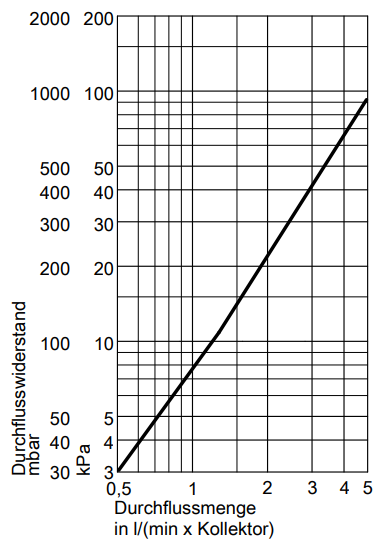
\includegraphics[width=0.65\textwidth]{Abbildungen/Druckverlust.png}
    \caption{Durchflusswiderstand Vitosol-FM/-F, Typ SV und SH\cite[S.129]{Viessmann}}
    \label{fig:Druckverlust}  
\end{figure}

\subsection{h}
Berechnen Sie nun den Druckverlust der Verrohrung des Solarkreises. Es wird ein neues Kupferrohr ein-
gesetzt. Die einfache Rohrleitungslänge (z. B. Vorlauf) beträgt 12 m. Den Druckverlust durch Einzelwi-
derstände und im Wärmeübertrager dürfen Sie dadurch berücksichtigen, dass Sie den Druckverlust der
Verrohrung um 45 \% erhöhen
\subsection{i}
Um die Anlagenkennlinie des Systems erstellen zu können, muss abschließend noch der
Gesamtdruckverlust $\Delta p_0$ aus der Summe der ermittelten Druckverluste berechnet werden
und dann entsprechend \autoref{eq:Kennlinie} die Kennlinie berechnet und erstellt werden.

\begin{equation}
    \label{eq:Kennlinie}
    \Delta p (\dot{V}) = \Delta p_0  \cdot \frac{\dot{V}}{ \dot{V_0} }
\end{equation}
\vspace{\baselineskip}
\begin{center}
    Gesamtdruckverlust $p_0 =p_r + p_{EW,WÜ} = 35048,28 Pa$\\
    Volumenstrom im Kollektorkreis $\dot{V_0} = 739,2\frac{l}{h}$
\end{center}
\section{Schwankungsbreite}
\label{sec:Schwankungsbreite}
\subsection{j}
Um die Auslegung des Systems zu vollenden, ist es notwendig neben der gemittelten
Variante auch die Extrema zu dimensionieren, um abschließend feststellen zu können, ob
Anpassungen am gemittelten System notwendig sind, um eine sichere Versorgung
gewährleisten zu können.\\
Das erste Extrema ist die Dimensionierung der Anlage bei maximaler Bestrahlung $E_{gen,max}$ und
minimalem jährlichen Gesamtwärmebedarf $Q_{Ges,min}$. Beim zweiten Extrema werden die jeweils entgegengesetzten
Werte genutzt.\\
Das erste Extrema benötigt 2 Kollektoren weniger, da bei höherem Ertrag je Kollektor weniger Wärme benötigt
wird. Es handelt sich also um die in diesem Rahmen bestmöglichen Umstände.
Daraus folgt ebenfalls, dass das Speichervolumen um 231 Liter sinkt und der kleiner Viessmann Vitocell 340-M Speicher
verwendet werden kann. Die Rohrleitung für beide Systeme wären DIN20-Rohre. Das führt dazu, dass der Volumenstrom
im Vergleich sinkt, die Strömung laminar wird und eine Verringerung des Gesamtdruckverlustes um rund 15000 Pa erwartbar ist.\\
Das zweite Extrema stellt insgesamt betrachtet den erwartbaren Worst Case dar.
Es würde 1 Kollektor mehr benötigt werden als beim gemittelten System. Beim Speicher würde weiterhin
der Viessmann Vitocell 360-M mit 950 Liter Fassungsvermögen genutzt werden, obwohl der errechnete Speicherraum
um 115,5 Liter auf 1039,5 Liter steigen würde. Hier gäbe es keine Änderung, da wir bei diesem Modell bereits den größten
Speicher des gewählten Herstellers nutzen. Die Rohrleitungen des Systems müssten auf DIN25 vergrößert werden, so
hätte das System trotz gestiegenem Volumenstrom eine Minderung des Gesamtdruckverlustes von rund 6800 Pa vorzuweisen.\\

\begin{figure}[H]
    \centering
    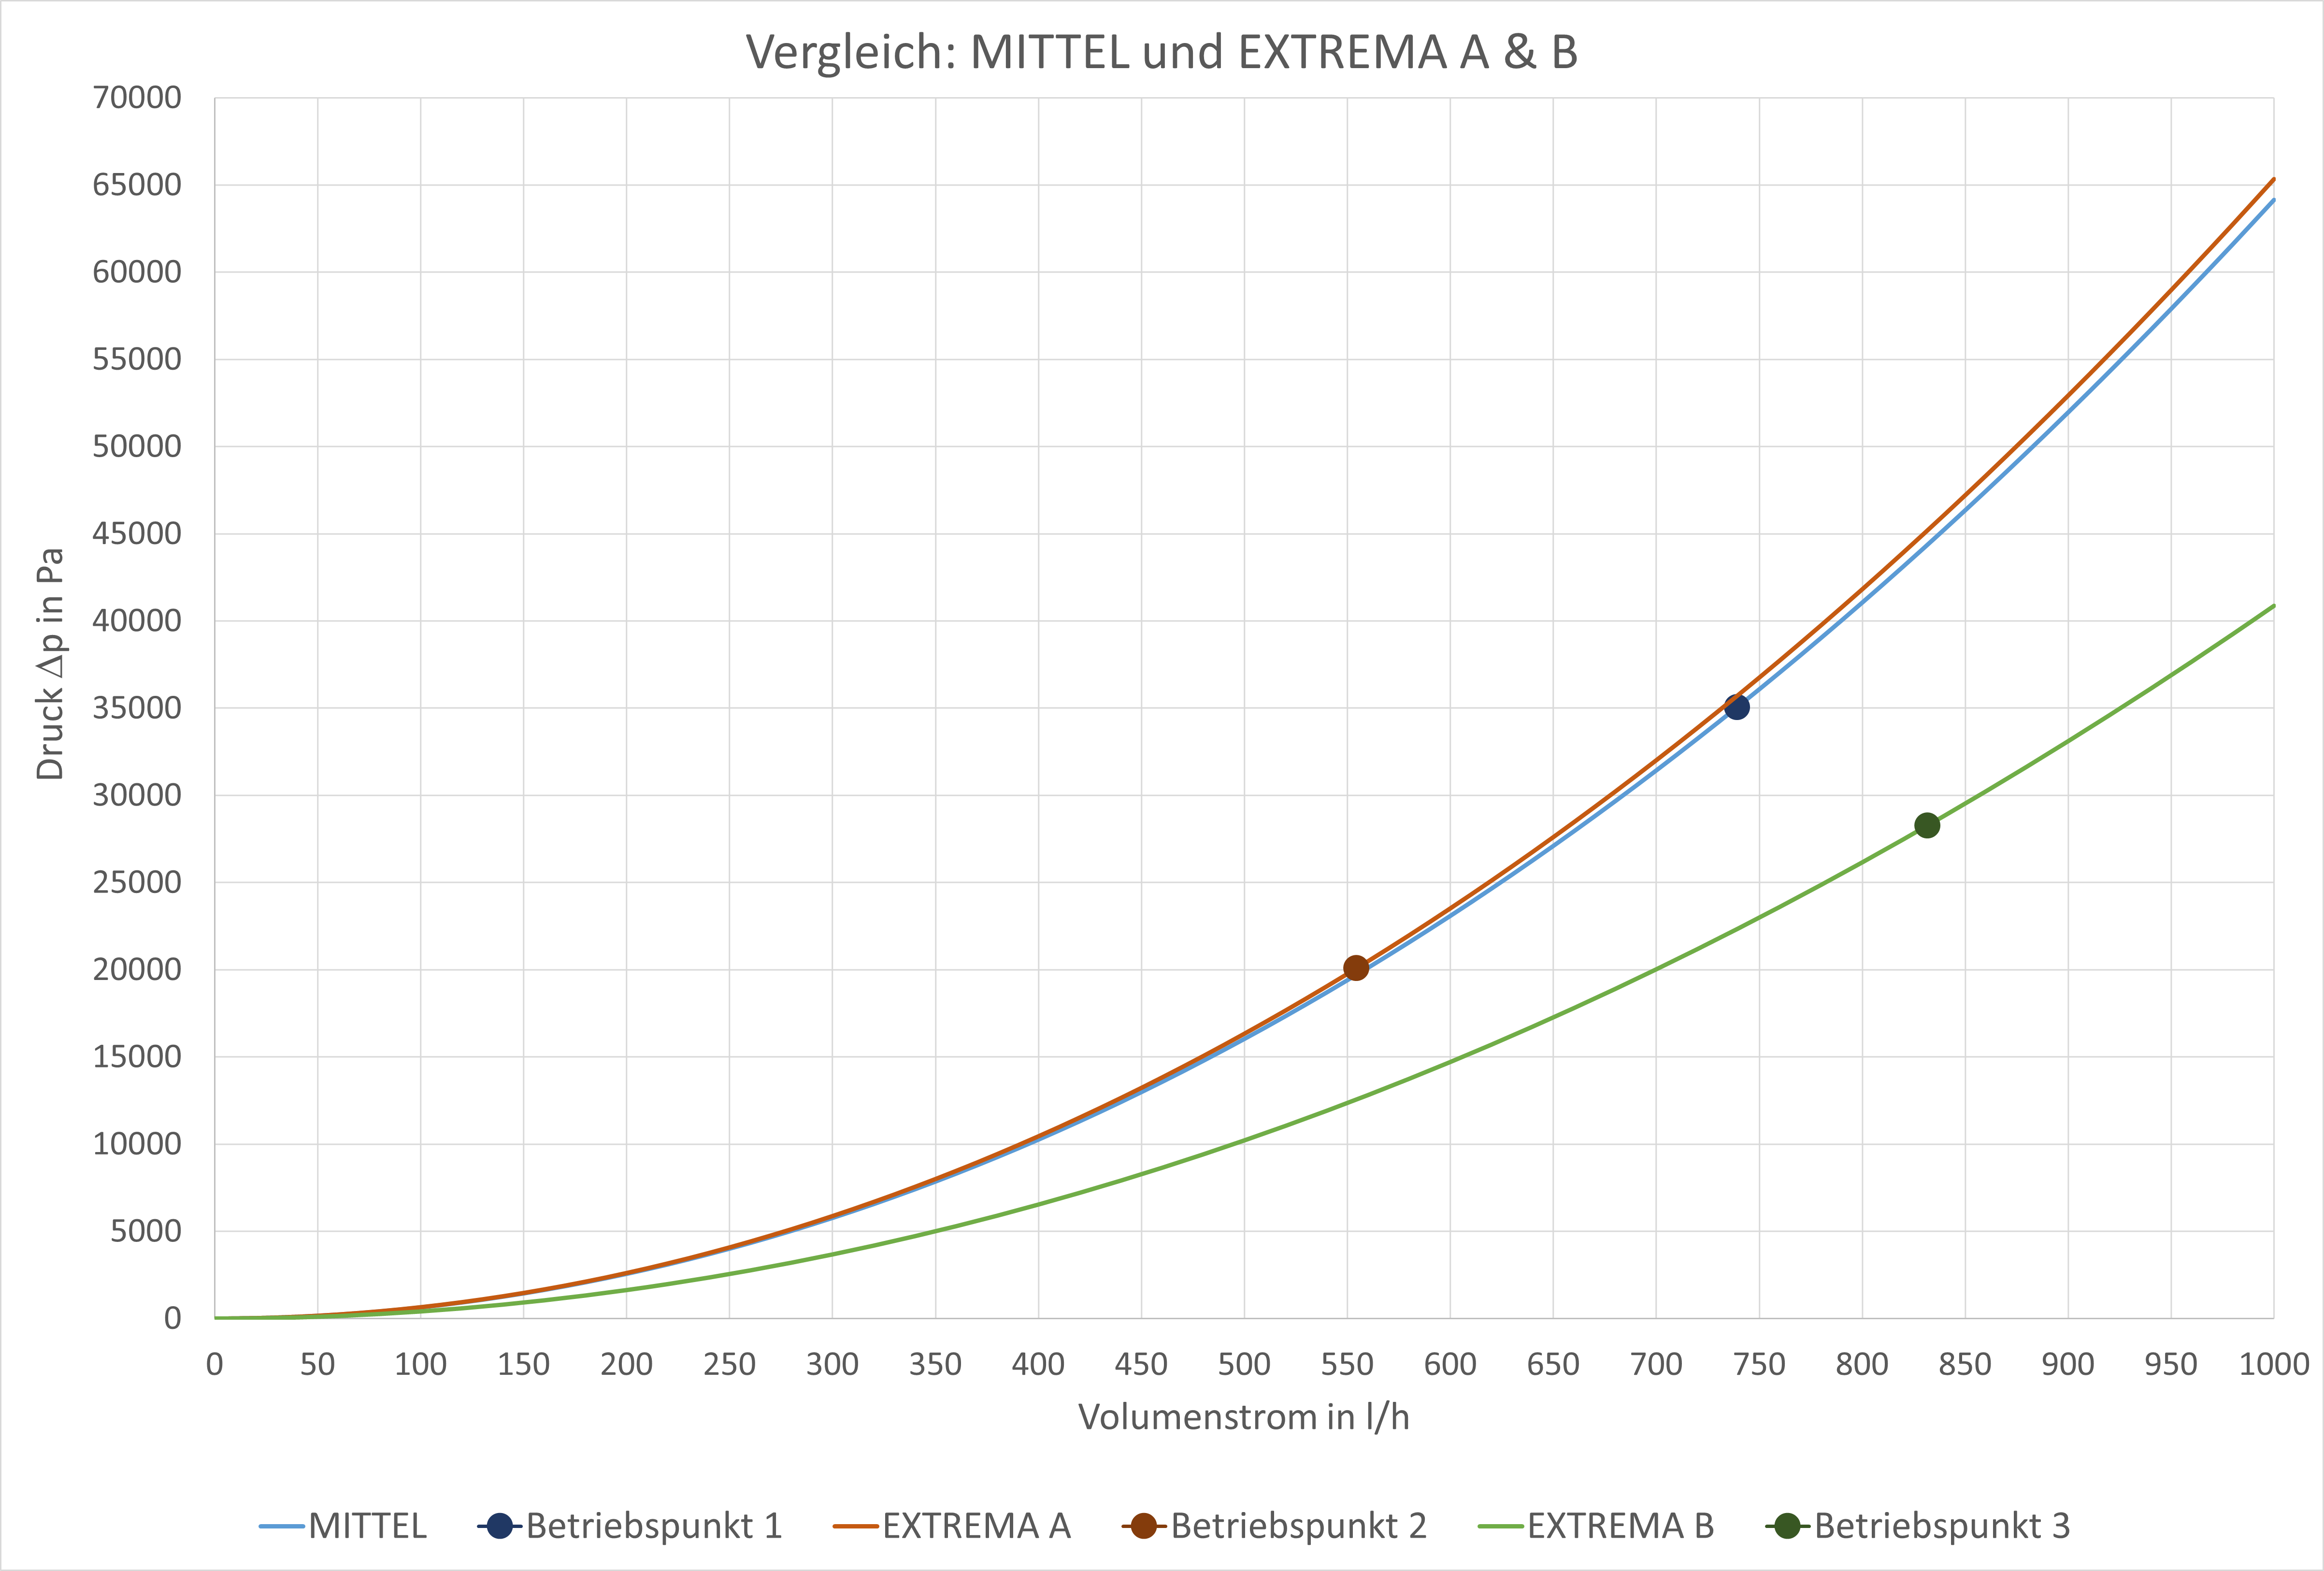
\includegraphics[width=\textwidth]{Abbildungen/Kennlinie-Vergleich.png}
    \caption{Vergleich der Kennlinien und Betriebspunkte aller Auslegungen}
    \label{Vergleich}
\end{figure}

Abschließend würde ich das System an das zweite Extrema anpassen.
Denn trotz der Mehrkosten für Kollektoren und Verrohrung wäre dieses System gegenüber den beiden
Anderen finanziell vorteilhafter, da so sichergestellt werden kann, dass auch bei schlechten Umständen der
solare Deckungsgrad auf min. 30\% gehalten wird und so eine Inbetriebnahme der Nachheizung außerhalb
der Heizperioden verhindert werden könnte. Zusätzlich kann im Vergleich zum Mittel-System in \autoref{sec:Pumpe}
ein kleineres und entsprechend preiswerteres Pumpenmodell gewählt werden.

\subsection{k}
(hierfür gibt es Bonuspunkte)
Recherchieren Sie und wählen Sie eine geeignete Pumpe für den Kollektorkreis aus, die Ihrer gewählten
Systemkonfiguration gerecht wird
\newpage
%Quellenverzeichnis
\sloppy
\bibliography{Sub-Files/Libs/Quellen.bib}
\fussy


\end{document}
